\documentclass{beamer}

\usepackage[T1]{fontenc}
\usepackage[latin1]{inputenc}
\usepackage[frenchb]{babel}
\usepackage{xcolor}
\usepackage{graphicx}
\usepackage{textpos}
\usepackage{subfig}

%\usetheme{Warsaw}
\usetheme[currentsection,hideothersubsections]{PaloAlto}
%\usetheme{Antibes}

\setbeamertemplate{navigation symbols}{}

\setbeamertemplate{itemize item}[triangle]

 %la barre d'info
    \setbeamercolor*{author in head/foot}{parent=palette tertiary}
    \setbeamercolor*{title in head/foot}{parent=palette secondary}
    \setbeamercolor*{date in head/foot}{parent=palette primary}
    \setbeamercolor*{page in head/foot}{parent=palette tertiary}
    \defbeamertemplate*{footline}{infolines theme}
    {
       \leavevmode%
         \hbox{%
           %\begin{beamercolorbox}[wd=.25\paperwidth,ht=2.25ex,dp=1ex,center]{author in head/foot}%
             %\usebeamerfont{author in head/foot}Une partie inutile
             %\end{beamercolorbox}%
             \begin{beamercolorbox}[wd=.77\paperwidth,ht=2.25ex,dp=1ex,center]{title in head/foot}%52
             \usebeamerfont{title in head/foot}\insertshorttitle
             \end{beamercolorbox}%
             \begin{beamercolorbox}[wd=.16\paperwidth,ht=2.25ex,dp=1ex,center]{date in head/foot}%
             \usebeamerfont{date in head/foot}\insertshortdate{}%\hspace*{2em}
           \end{beamercolorbox}%
           \begin{beamercolorbox}[wd=.08\paperwidth,ht=2.25ex,dp=1ex,center]{page in head/foot}
            \insertframenumber/\inserttotalframenumber
           \end{beamercolorbox}%
         }%
    }


\hypersetup{
    pdfauthor   = {Benoit Meilhac},%
    pdftitle    = {Projet Yuukou II},%
    pdfsubject  = {Soutenance de stage},%
    pdfkeywords = {soutenance, Yuukou II, service Web, Westminster},%
    pdfcreator  = {PDFLaTeX},%
    pdfproducer = {PDFLaTeX}%
}

\graphicspath{{images/}}

\logo{
	%
\includegraphics[width=1.5cm]{westminsterLogo.jpg}
}

\title[Projet Yuukou II]{
    Projet Yuukou II
}

\institute{
	
\includegraphics[scale=0.5]{femtoLogo.jpg}

	\begin{center}
		\textsc{MEILHAC Beno\^it}\\

	\end{center}

	Tuteur de stage : M. Thierry DELAITRE\\
	Responsable de stage : M. Jean-Michel HUFFLEN
}

\date[11 juin 2012]{}

\author[]{ 
	Universit\'e de France-Comt\'e\\
	D\'epartement informatique\\
}

\begin{document}

\begin{frame}
    	\titlepage

\end{frame}

\section*{Sommaire}

\begin{frame}{Sommaire}
	\tableofcontents[hideallsubsections]

\end{frame}

\section{Lieu du stage}

\begin{frame}{University of Westminster}
	\begin{block}{Pr\'esentation}
		\begin{itemize}
			\item Universit\'e publique de recherche situ\'e \`a Londres
			\item Fond\'ee en 1838 comme la \textit{Royal Polytechnic Institution}
			\item 4 grands campus et 2 plus petits dans Londres et ses alentours
			\item Plus de 20 000 \'etudiants de 150 nations diff\'erentes
			\item Grands noms comme Sir Alexander Fleming ou Christopher Bailey

		\end{itemize}

	\end{block}

	\begin{block}{School of Electronics and Computer Science}
		\begin{itemize}
			\item 101-115 New Cavendish Street dans le quartier de Fitzrovia
			\item Divers parcours de l'ing\'enierie informatique et \'electronique aux math\'ematiques appliqu\'ees

		\end{itemize}

	\end{block}

\end{frame}

%%%%%%%%%%%%%%%%%%%%%%%%%%%%%%%%%

\begin{frame}{University of Westminster}
	\begin{block}{\'Equipes int\'egr\'ees}
		\begin{itemize}
			\item \textit{Information Systems and Library Services} (ISLS)
			\begin{itemize}
				\item Services centraux informatiques
				\item Gestion de tout ce qui touche \`a l'\'education : acc\`es au mat\'eriel  informatique, aux archives, \ldots

			\end{itemize}

			\item \textit{Infrastructure Team}
			\begin{itemize}
				\item Gestion des laboratoires informatiques sp\'ecialis\'es
				\item 34 laboratoires et 13 personnes
				\item \'Etend des services fournis par ISLS

			\end{itemize}

		\end{itemize}

	\end{block}

\end{frame}

%%%%%%%%%%%%%%%%%%%%%%%%%%%%%%%%%

\begin{frame}{University of Westminster}
	\begin{block}{\textit{Centre for Parallel Computing}  (CPC)}
		\begin{itemize}
			\item Lieu de travail pendant les 4 mois
			\item Recherche dans la technologie et les applications de calculs parall\`els et distribu\'es
			\item Gemlca, NGS, SHIWA, \ldots

		\end{itemize}

	\end{block}

\end{frame}

\chapter{Pr\'esentation du sujet}

\section{Le projet \Yuukou}

\begin{figure}[!ht]
	\centering
	
\includegraphics[scale=1]{yuukouLogo.jpg}

\end{figure}

\subsection{Pr\'esentation}

Le terme Yuukou comme abord\'e dans l'introduction de ce rapport, vient du japonais \Yuukou{} et signifie validit\'e, disponibilit\'e, efficacit\'e.
C'est un syst\`eme permettant la r\'ecup\'eration des informations depuis les serveurs LDAP\protect\footnote{\textit{Lightweight Directory Access Protocol}}$^*$ de l'Universit\'e afin de comprendre et construire l'infrastructure des ressources et ainsi de voir sa facilit\'e d'utilisation. 
L'architecture du syst\`eme utilise un processus d'apprentissage simple pour d\'eduire et maintenir la structure \`a jour avec un minimum de r\'eglages initiaux.
\Yuukou{} a \'et\'e cr\'e\'e pour montrer l'utilisation des salles informatiques et conserver un historique des informations sur le campus de New Cavendish.

\subsection{Fonctionnement}

Le but principal de \Yuukou{} est d'afficher l'occupation des salles informatiques en se rapprochant autant que possible du comportement d'un syst\`eme fonctionnant en temps r\'eel.
Pour ce faire, l'application a \'et\'e divis\'ee en deux parties  comme le montre la figure~\ref{figure:yuukouFonctionnement}.

\clearpage

\begin{figure}[!ht]
	\centering
	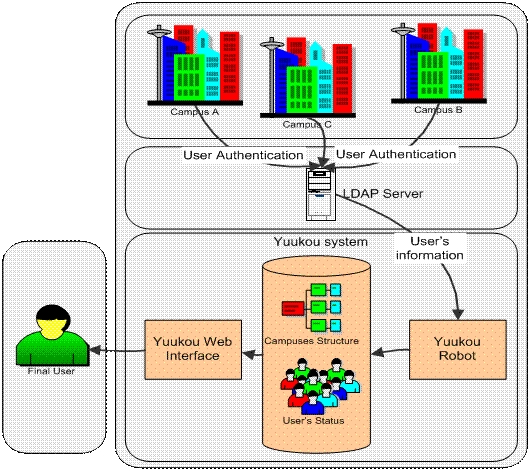
\includegraphics[scale=0.75]{yuukouFonctionnement.jpg}
	\caption{Architecture de \Yuukou}
	\label{figure:yuukouFonctionnement}

\end{figure}

\subsubsection{Premi\`ere partie}

La premi\`ere partie est un programme \'ecrit en Perl$^*$ qui r\'ecup\`ere les informations de connexion des utilisateurs depuis un serveur LDAP$^*$ et qui se charge de construire, modifier ou mettre \`a jour l'architecture r\'eseau de l'Universit\'e tout en stockant les informations dans une base de donn\'ees relationnelle de type MySQL.

Le robot de \Yuukou{} offre deux fonctionnalit\'es : il permet de mettre \`a jour les donn\'ees de connexion \textit{via} le serveur LDAP$^*$ toutes les cinq minutes environ pour une utilisation normale, et de mettre \`a jour le statut des ressources (ordinateurs) toutes les demi-heures, l\`a aussi pour une utilisation normale.

\subsubsection{Deuxi\`eme partie}

La seconde partie est un ensemble de pages Web \'ecrites en PHP\protect\footnote{\textit{Personal Home Page} ou \textit{PHP: Hypertext Preprocessor}}$^*$ et h\'eberg\'ees sur un serveur Web permettant de pr\'esenter les donn\'ees collect\'ees \`a l'utilisateur final.
Ces pages sont de deux types : les pages publiques et les pages priv\'ees.

Les pages publiques sont accessibles par tous les utilisateurs de l'Universit\'e le d\'esirant.
Les pages priv\'ees, quant \`a elles, ne sont accessibles qu'aux administrateurs.

\subsubsection{Les pages publiques}

\noindent Les pages publiques permettent l'affichage des pages suivantes :

\begin{itemize}
	\item une page contenant tous les campus et salles informatiques actuellement utilis\'ees;
	\item une page par campus avec les salles informatiques actuellement utilis\'ees;
	\item une page par campus et d\'epartement avec les salles informatiques actuellement utilis\'ees.

\end{itemize}

\vspace{0.20cm}

Les pages publiques offrent une vision g\'en\'erale de chaque salle : le nombre de ressources totales, disponibles, occup\'ees par un utilisateur et dans un \'etat inconnu.
Il est \`a noter que chacunes des pr\'ec\'edentes pages peut \^etre affich\'ees sur un \'ecran plasma pr\'esent dans les diff\'erents b\^atiments de l'Universit\'e.
La figure~\ref{figure:yuukouPublic} donne un exemple de page publique.

\subsubsection{Les pages priv\'ees}

\noindent Les pages priv\'ees permettent l'affichage des pages suivantes :

\begin{itemize}
	\item une page d'identification \textit{via} LDAP$^*$ pour l'administrateur;
	\item toutes les pages publiques mais b\'en\'eficiant de fonctionnalit\'es suppl\'ementaires :

	\begin{itemize}
		\item liste des ressources \'eteintes;
		\item une fen\^etre permettant d'avoir des informations sur un utilisateur actuellement connect\'e \`a une ressource (identifiant, nom, photo, heure de connexion et dur\'ee de la session);
		\item possibilit\'e d'ajouter des commentaires sur les utilisateurs;
		\item liens vers les statistiques des salles informatiques.

	\end{itemize}

\end{itemize}

\vspace{0.20cm}

La figure~\ref{figure:yuukouAdmin} donne un exemple des fonctionnalit\'es suppl\'ementaires auxquelles un administrateur a acc\`es.

\clearpage

\subsubsection{Vue sur le produit}

\begin{figure}[!ht]
	\centering
	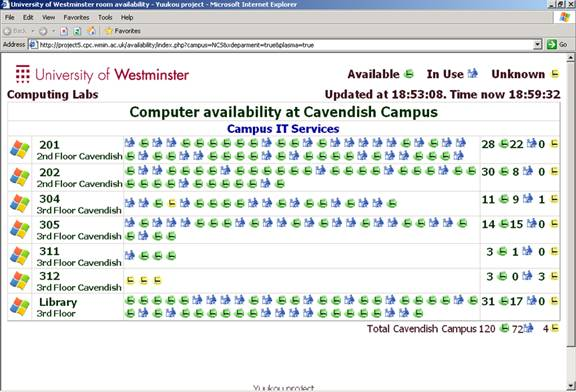
\includegraphics[scale=0.75]{yuukouPublic.jpg}
	\caption{Exemple de page publique de \Yuukou{} rep\'esentant un campus et l'utilisation des salles informatiques d'un d\'epartement}
	\label{figure:yuukouPublic}

\end{figure}

\begin{figure}[!ht]
	\centering
	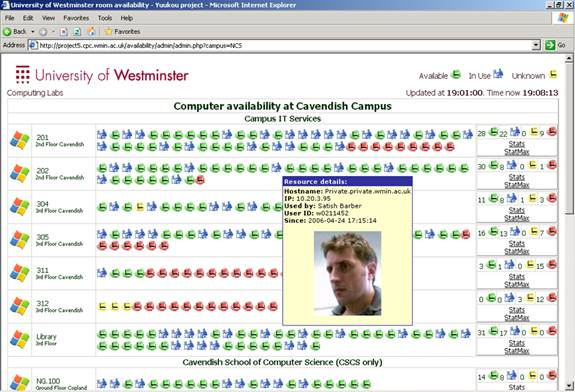
\includegraphics[scale=0.75]{yuukouAdmin.jpg}
	\caption{Exemple de page priv\'ee de \Yuukou{} montrant en particulier les donn\'ees d'un utilisateur}
	\label{figure:yuukouAdmin}

\end{figure}

\subsection{Quelques chiffres}

Le projet \Yuukou{} permet de surveiller le r\'eseau du campus de New Cavendish soit 43 salles informatiques, ce qui repr\'esente 661 PC. 
Le support des Macintosh n'\'etant pas pris en compte.

\subsection{Changement vers \YuukouII}

L'Universit\'e souhaite reprendre le principe du projet \Yuukou, cependant elle est confront\'ee \`a diff\'erents probl\`emes.
Le premier \'etant que les personnes ayant d\'evelopp\'e le projet ont quitt\'e l'Universit\'e. 
Ce qui signifierait, pour la personne ou l'\'equipe qui serait en charge de reprendre le projet, de prendre du temps pour se former \`a Perl$^*$, comprendre tout ce qui a \'et\'e d\'ej\`a r\'ealis\'e et ensuite seulement, commencer \`a d\'evelopper.
Actuellement de nombreux projets sont en cours et il n'est pas possible pour une \'equipe de passer du temps sur l'existant.

Un autre probl\`eme est les changements importants, du point de vue infrastructure, qui sont en train d'\^etre mis en place.
En effet, l'Universit\'e qui utilisait eDirectory$^*$ de Novell pour g\'erer ses annuaires LDAP$^*$ a commenc\'e \`a migrer toutes ses donn\'ees vers le syst\`eme Active Directory$^*$ de Microsoft qui est cens\'e \^etre plus efficace. Ce changement rendrait \Yuukou{} obsol\`ete.

Point suivant, la volont\'e de donner acc\`es aux informations sur les salles, pas seulement en utilisant un navigateur Internet, mais aussi et surtout en utilisant un \textit{smartphone} (IPhone ou autre par exemple) ou une tablette (IPad par exemple), chose que l'ancien logiciel ne peut pas fournir.
De ce fait, un \'etudiant aurait \`a tout moment les informations sur les salles \textit{via} son \textit{smartphone} ou sa tablette, si tant est qu'il ait l'un ou l'autre.

\noindent \`A ces pr\'ec\'edents probl\`emes, d'autres viennent s'ajouter :

\begin{itemize}
	\item les Macintosh ne sont pas pris en compte;
	\item le logiciel est assez monolithique, il deviendrait donc tr\`es difficile et complexe de vouloir l'\'etendre;
	\item {\Yuukou} ne prend en compte que les donn\'ees en temps r\'eel et ne garde pas un historique;
	\item son utilisation pr\^ete \`a confusion car il n'a aucun interfa\c{c}age avec l'emploi du temps, de ce fait, quand une salle est pr\'esent\'ee comme libre, il n'y a aucun moyen, avec le logiciel, de savoir si un cours s'y d\'eroule ou non.

\end{itemize}

\vspace{0.20cm}

C'est en consid\'erant tous ces points qu'il a \'et\'e d\'ecid\'e d'abandonner le projet \Yuukou{} afin de pouvoir mettre en place \YuukouII{} qui r\'epondrait aux attentes de l'Universit\'e.

\section{Le projet \YuukouII}

{\YuukouII} a pour but de combler les lacunes de {\Yuukou} et d'aller plus loin en termes de fonctionnalit\'es qu'il peut offrir. 
Le projet sera tout d'abord pr\'esent\'e avec les principaux points le composant.
Ensuite seront abord\'ees les diff\'erentes r\'eflexions que les \'equipes int\'eress\'es par le projet ont effectu\'ees.
Ces r\'eflexions donneront lieu aux premi\`eres id\'ees qui en ont \'emerg\'ees.
Enfin, les principales contraintes techniques du projet seront d\'ecrites.

\subsection{Pr\'esentation du projet}

Dans son fonctionnement g\'en\'eral, {\YuukouII} doit permettre de donner \`a un \'etudiant ou toute personne travaillant \`a l'Universit\'e et cherchant \`a utiliser un ordinateur, une vue globale des ressources qui sont disponibles actuellement.
Les donn\'ees devant \^etre bien s\^ur exactes afin que la personne n'ait pas de mauvaise surprise en se rendant dans une salle qu'elle pensait libre.
L'affichage pourra se faire \textit{via} un \textit{smartphone}, une tablette ou encore un navigateur Internet.

\noindent Le but du stage est : 

\begin{itemize}
	\item la conception d'un logiciel permettant la r\'ecup\'eration de donn\'ees concernant les connexions sur les diff\'erentes ressources de l'Universit\'e et cela en temps r\'eel;
	\item la gestion de la persistance de ces donn\'ees;
	\item la cr\'eation d'un maximum de fonctionnalit\'es retournant les informations utiles dans le but d'\^etre exploit\'ees pour l'affichage sur les diff\'erents supports.

\end{itemize} 

\vspace{0.20cm}

La cr\'eation d'applications permettant l'affichage des r\'esultats ne fait pas partie de ce sujet de stage. 
Ici, seule la partie r\'ecup\'eration, stockage et retour des donn\'ees est abord\'ee.

\subsection{R\'eflexions de l'\'equipe technique}

Diff\'erents acteurs de l'Universit\'e int\'eress\'es dans le projet \YuukouII{} ont commenc\'e \`a fixer une liste des fonctionnalit\'es qu'ils aimeraient voir avec l'application finale.

\subsubsection{Concernant les ressources}

\begin{itemize}
	\item Macintosh et Windows;
	\item conna\^itre l'\'etat de la ressource, \'eventuellement la d\'emarrer \`a distance (WOL\protect\footnote{\textit{Wake On Lan}}$^*$);
	\item inclure une surveillance partielle du mat\'eriel et des logiciels;
	\item utilisation des services d'Active Directory$^*$.

\end{itemize}

\subsubsection{Concernant les donn\'ees r\'ecup\'er\'ees}

\begin{itemize}
	\item mettre au point un formalisme avec les autres services de l'Universit\'e concernant les informations sur les salles, campus et d\'epartements;
	\item stocker les informations dans une base de donn\'ees SQL\protect\footnote{\textit{Structured Query Language}}$^*$;
	\item mettre en place des outils pour g\'en\'erer des statistiques \`a partir des donn\'ees stock\'ees (utilisation d'une salle, nombre de connexions par jour dans un mois pour une salle, \ldots).

\end{itemize}

\subsubsection{Concernant les donn\'ees retourn\'ees}

\begin{itemize}
	\item g\'en\'eration de flux RSS\protect\footnote{\textit{Rich Site Summary}}$^*$ pour retourner des informations;
	\item l'affichage doit \^etre en temps r\'eel et doit aussi permettre d'avoir une vue globale dans le temps : utilisation des emplois du temps pour savoir quelle salle est libre et \`a quel moment.

\end{itemize}

\vspace{0.20cm}

Cette liste n'est pas compl\`ete \'etant donn\'e qu'elle ne prend pas en compte la partie \og{}affichage\fg{} des r\'esultats du fait que le projet ne consiste qu'\`a la r\'ecup\'eration, au traitement et au retour de donn\'ees.

L'id\'ee initiale \'etait de d\'evelopper un projet pilote qui permettrait d'avoir une vue sur ce qu'il est possible de faire et sur la fa\c{c}on de le faire.
Il serait ensuite repris par les \'equipes de l'Universit\'e pour \^etre termin\'e.
Ce projet consisterait en la cr\'eation d'un service Web (la notion sera expliqu\'ee plus en d\'etail au \S~\ref{section:serviceWeb}) \'ecrit en C\# et utilisant le \textit{framework}$^*$ .Net de Microsoft.
Le service Web devra offrir un maximum de fonctionnalit\'es et \^etre exploit\'e par une application mobile pour \textit{smartphone} et par un site Web pouvant \^etre projet\'e sur les \'ecrans plasma \`a l'entr\'ee de chaque site.

Cependant, apr\`es r\'eflexion avec M. Thierry DELAITRE, la structure, les objectifs et le projet en g\'en\'eral ont \'et\'e revus.
Dans l'id\'ee initiale, pour conna\^itre l'\'etat d'une ressource, si elle est \'eteinte ou allum\'ee par exemple, il aurait fallu interroger Active Directory$^*$. 
De plus, n'est connu que l'\'etat si un utilisateur est connect\'e.
Il faudrait des traitements suppl\'ementaires pour pouvoir fixer pr\'ecisement l'\'etat d'une ressource, avec un \textit{ping} par exemple pour savoir si la ressource est \'eteinte ou non.

\subsection{Premi\`eres approches}

Une solution simple, rapide et fonctionnelle avait d\'ej\`a \'et\'e mise en place afin de \og{}monitorer\fg{}, \cad{} surveiller le fonctionnement des diff\'erentes ressources de certaines salles dans l'Universit\'e.
Nagios est une application permettant d'effectuer une surveillance syst\`eme et r\'eseau.
Il permet de conna\^itre l'\'etat d'une machine ainsi que d'autres informations comme le syst\`eme d'exploitation utilis\'e, la version de Java install\'ee, la charge du processeur, \ldots

En partant de ce logiciel, le projet consiste en la r\'ecup\'eration des donn\'ees de Nagios, leur traitement et le d\'eveloppement des fonctionnalit\'es permettant \`a une application ext\'erieure de pouvoir afficher les informations.

\noindent Les objectifs principaux deviennent les suivants :

\begin{itemize}
	\item cr\'eation d'un service Web en utilisant l'API\protect\footnote{\textit{Application Programming Interface}}$^*$ Java JAX-WS\protect\footnote{\textit{Java API for XML Web Services}};
	\item mise en place d'une m\'ethode de communication avec Nagios;
	\item cr\'eation de la base de donn\'ees permettant l'archivage;
	\item mise en place d'un cycle permettant de traiter les informations r\'ecup\'er\'ees;
	\item d\'efinition de fonctions utiles pour une application cliente;
	\item choix d'une structure de retour des informations pour une application cliente;
	\item faire un lien avec l'emploi du temps des diff\'erentes salles sous surveillance.

\end{itemize}

\subsection{Contraintes techniques}

Deux des principales contraintes du cahier des charges sont l'utilisation de logiciels libres et du langage de d\'eveloppement Java, tout en me laissant un maximum de libert\'e dans les autres choix.

Durant le stage, un ordinateur m'a \'et\'e fourni avec un libre choix sur le syst\`eme d'exploitation.
De ce fait j'ai opt\'e pour un Linux Mint 11 nomm\'e \textit{Katya}, que j'ai l'habitude d'utiliser.

Un autre ordinateur, lui contenant un Debian 6.0.5 nomm\'e \textit{Squeeze}, a \'et\'e mis \`a ma disposition en tant que serveur distant h\'ebergeant le service Web ainsi que les diff\'erents outils n\'ecessaires \`a son fonctionnement.
Le serveur distant contient le logiciel Nagios, le serveur Web permettant de faire fonctionner la derni\`ere version stable du service Web ainsi que le syst\`eme de gestion de bases de donn\'ees (SGBD).

Les tests \'etant en premier lieu r\'ealis\'es en local sur la machine de d\'eveloppement et ensuite, quand le fonctionnement \'etait garanti, l'application \'etait d\'eploy\'ee sur le serveur distant.
Des renseignements suppl\'ementaires seront apport\'es au \S~\ref{section:gestionProjet}.


\clearpage

\section{Premi\`eres approches}

\subsection{Notion de service Web}

\begin{frame}{Notion de service Web}
	\begin{block}{D\'efinition}
		\begin{itemize}
			\item Application accessible par le r\'eseau
			\item Ind\'ependant de tous langages
			\item Communication avec un client
			
		\end{itemize}
		
	\end{block}
	
	\begin{block}{Architecture}
		\begin{itemize}
			\item Architecture SOA : distributions de services
			\item \'Echanges : SOAP
			\item Description : WSDL
			\item D\'ecouverte : UDDI

		\end{itemize}
		
	\end{block}
	
\end{frame}

%%%%%%%%%%%%%%%%%%%%%%%%%%%%%%%%%

\begin{frame}{Notion de service Web}
	\begin{figure}[h]
		\centering
		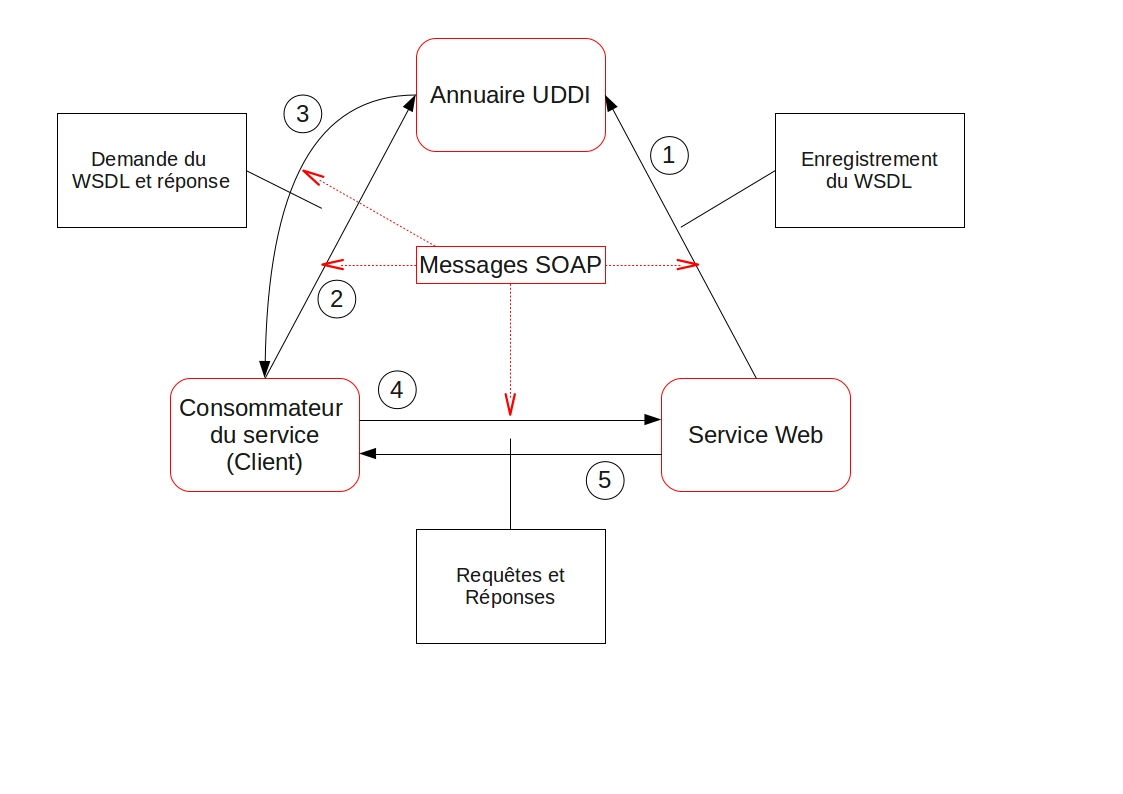
\includegraphics[scale=0.30]{schemaServiceWeb.jpg}
		
	\end{figure}
		
\end{frame}

%%%%%%%%%%%%%%%%%%%%%%%%%%%%%%%%%

\begin{frame}{Notion de service Web}
	\begin{block}{API JAX-WS}
		\begin{itemize}
			\item API Java pour les services Web
			\item Diff\'erentes m\'ethodes de d\'eveloppememt
			\item Facilit\'e avec NetBeans et GlassFish
		
		\end{itemize}

	\end{block}

\end{frame}

%%%%%%%%%%%%%%%%%%%%%%%%%%%%%%%%%

\subsection{Architecture du projet}

\begin{frame}{Architecture du projet}
	\begin{figure}[h]
		\centering
		\only<1>{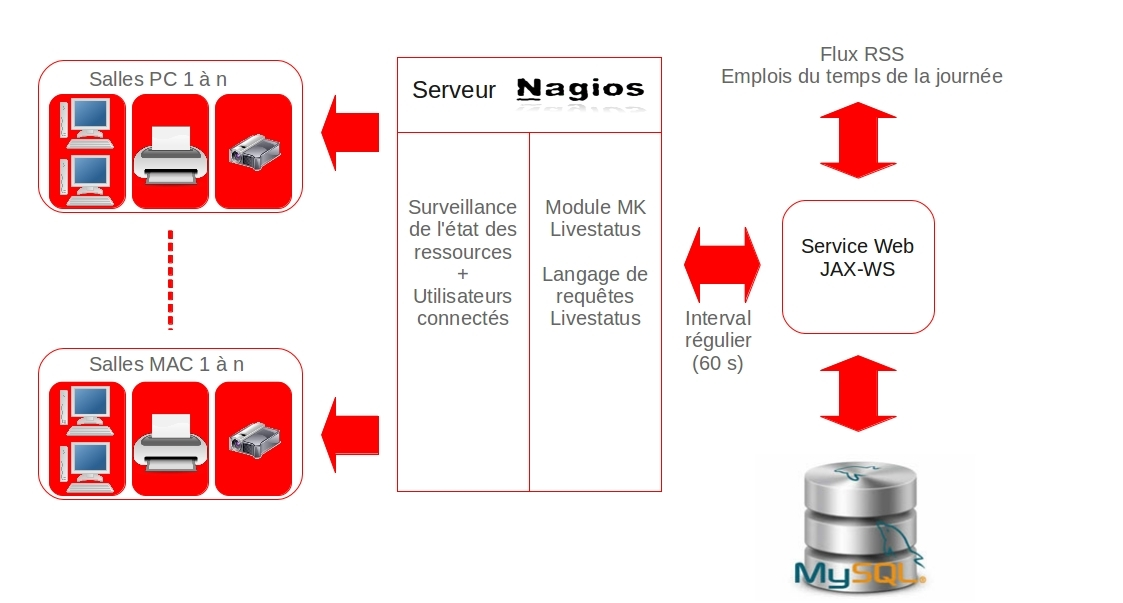
\includegraphics[scale=0.30]{architectureProjetServiceWeb.jpg}}
		\only<2>{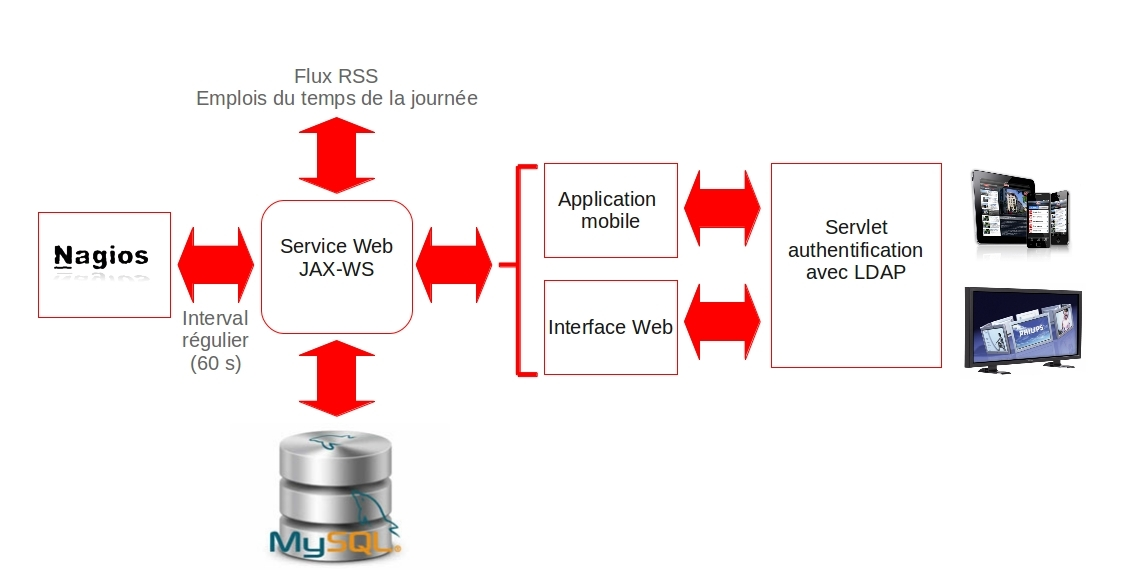
\includegraphics[scale=0.275]{architectureProjetAffichage.jpg}}
			
	\end{figure}
	
\end{frame}

%%%%%%%%%%%%%%%%%%%%%%%%%%%%%%%%%

\subsection{Outils utilis\'es}

\begin{frame}{Surveillance des ordinateurs}
	\begin{figure}[h]
		\centering
		
\includegraphics[scale=0.30]{nagiosLogo.jpg}
			
	\end{figure}
	
	\begin{block}{Nagios}
		\begin{itemize}
			\item Surveillance syst\`eme et r\'eseau
			\item Logiciel libre
			\item Interface graphique
		
		\end{itemize}

	\end{block}
	
\end{frame}

%%%%%%%%%%%%%%%%%%%%%%%%%%%%%%%%%

\begin{frame}{Surveillance des ordinateurs}
	\begin{block}{Module MKLivestatus}
		\begin{itemize}
			\item Int\'egr\'e au processus de Nagios
			\item Socket de communication
			\item \textit{Livestatus Query Language}
		
		\end{itemize}

	\end{block}
	
	\begin{block}{Quelques chiffres}
		\begin{itemize}
			\item Initialement
			\begin{itemize}
				\item Campus de New Cavendish
				\item 31 salles informatiques
				\item Environ 600 PC
			
			\end{itemize}
			
			\item Actuellement
			\begin{itemize}
				\item Presque toutes les salles
				\item 102 salles informatiques dont 3 pour les MAC
				\item 1920 PC et 63 MAC
			
			\end{itemize}
		
		\end{itemize}

	\end{block}
	
\end{frame}

%%%%%%%%%%%%%%%%%%%%%%%%%%%%%%%%%

\begin{frame}{Autres outils}
	\begin{figure}[h]
		\centering
		\subfloat{
\includegraphics[scale=0.242]{netbeansLogo.jpg}}
		\qquad
		\subfloat{
\includegraphics[scale=0.242]{glassfishLogo.jpg}}
		\qquad
		\subfloat{
\includegraphics[scale=0.3]{mysqlLogo.jpg}}

	\end{figure}

	\begin{block}{Autres outils}
		\begin{itemize}
			\item IDE NetBeans
			\item Serveur d'application GlassFish
			\item SGBD MySQL
		
		\end{itemize}

	\end{block}
	
\end{frame}

%%%%%%%%%%%%%%%%%%%%%%%%%%%%%%%%%

\begin{frame}{Choix du format de retour du service Webl}
	\begin{block}{Les recherches}
		\begin{itemize}
			\item Texte structur\'e
			\item Objet s\'erialisable
			\item XML
			\item JSON
		
		\end{itemize}

	\end{block}
	
	\begin{block}{Le choix}
		\begin{itemize}
			\item JSON
			\item Simple et rapide
			\item Langage d'\'echange id\'eal
		
		\end{itemize}

	\end{block}

\end{frame}



\subsection{Organisation du travail}

\begin{frame}{Organisation du travail}
	\begin{figure}[h]
		\centering
		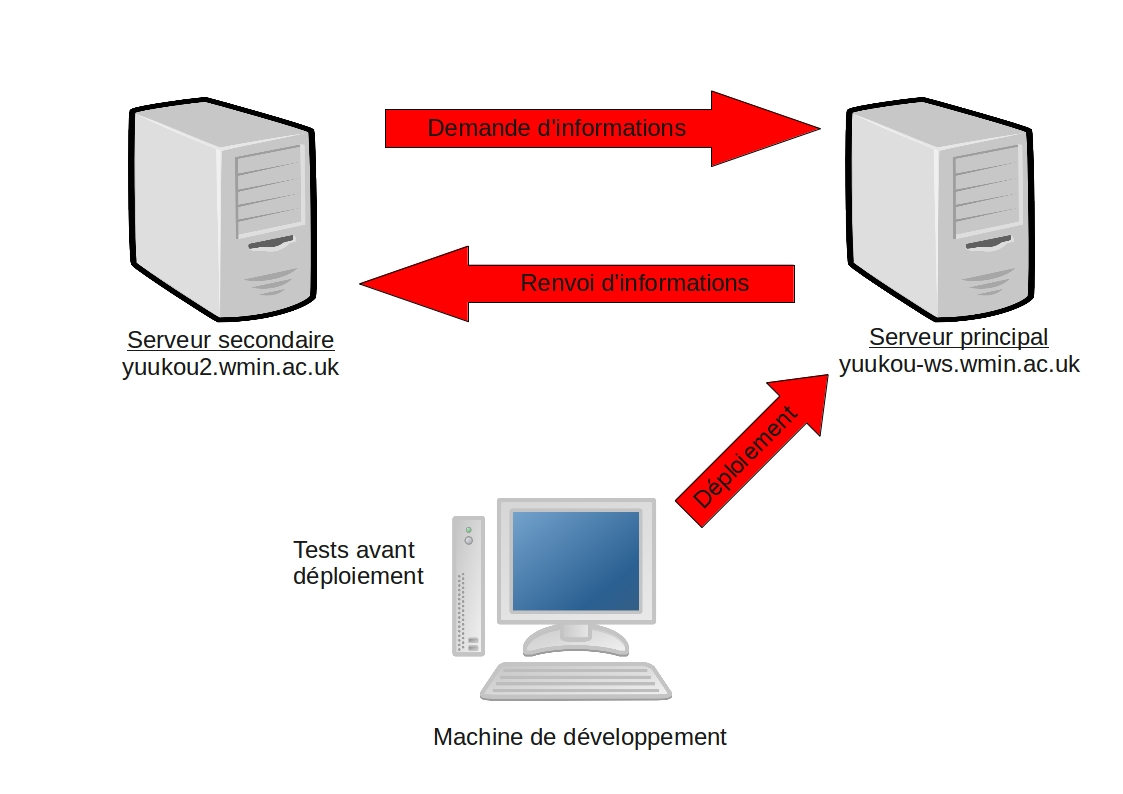
\includegraphics[scale=0.242]{gestionProjet.jpg}

	\end{figure}

\end{frame}
















\section{Le service Web de Yuukou II}

\subsection{Cycle Principal}

\begin{frame}{Cycle principal}
	\begin{block}{Fonctionnement}
		\begin{itemize}
			\item R\'ecup\'eration des donn\'ees Nagios
			\item V\'erifications sur les donn\'ees
			\item Ajout/mise \`a jour/effacement dans la base de donn\'ees
			\begin{itemize}
				\item Ordinateurs
				\item Utilisateurs avec LDAP
				\item Couples ordinateur-utilisateur : archivage d'utilisation
				\item Emplois du temps
			
			\end{itemize}
			
			\item Toutes les minutes

		\end{itemize}

	\end{block}

\end{frame}

%%%%%%%%%%%%%%%%%%%%%%%%%%%%%%%%%

\subsection{Retours client}

\begin{frame}{Retours client}
	\begin{block}{Fonctions publiques}
		\begin{itemize}
			\item Fonctions simples
			\item \'Etats et informations des salles informatiques
			
		\end{itemize}

	\end{block}
	
	\begin{block}{Fonctions priv\'ees}
		\begin{itemize}
			\item Compl\'ements aux fonctions publiques
			\item Gestion du service Web 
			\item Fonctions avanc\'ees
			
		\end{itemize}

	\end{block}

\end{frame}

%%%%%%%%%%%%%%%%%%%%%%%%%%%%%%%%%

\subsection{Fonctionnalit\'es}

\begin{frame}{Fonctionnalit\'es du service Web}
	\begin{block}{S\'ecurisation}
		\begin{itemize}
			\item SSL
			\item Certificats fournis par l'Universit\'e
			
		\end{itemize}

	\end{block}
	
	\begin{block}{G\'en\'eration de statistiques}
		\begin{itemize}
			\item API RRD4J
			\item Graphes d'utilisations des salles informatiques
			
		\end{itemize}

	\end{block}
	
	\begin{block}{Emplois du temps}
		\begin{itemize}
			\item 4 Flux RSS de l'Universit\'e
			\item Correspondance des noms des salles avec le projet
			
		\end{itemize}

	\end{block}
	
\end{frame}

%%%%%%%%%%%%%%%%%%%%%%%%%%%%%%%%%
	
\begin{frame}{Fonctionnalit\'es du service Web}
	\begin{block}{Catalogue logiciels}
		\begin{itemize}
			\item \textit{MediaWiki} pour la \textit{School of Electronics and Computer Science}
			\item Construction des diff\'erents liens
			
		\end{itemize}

	\end{block}
	
	\begin{block}{Gestion des donn\'ees}
		\begin{itemize}
			\item 50 000 \`a 60 000 donn\'ees par mois
			\item D\'eplacement mensuel des donn\'ees d'utilisation
			
		\end{itemize}

	\end{block}

\end{frame}

%%%%%%%%%%%%%%%%%%%%%%%%%%%%%%%%%

\begin{frame}{Utilisation par un client}
	\begin{figure}[h]
		\centering
		\subfloat{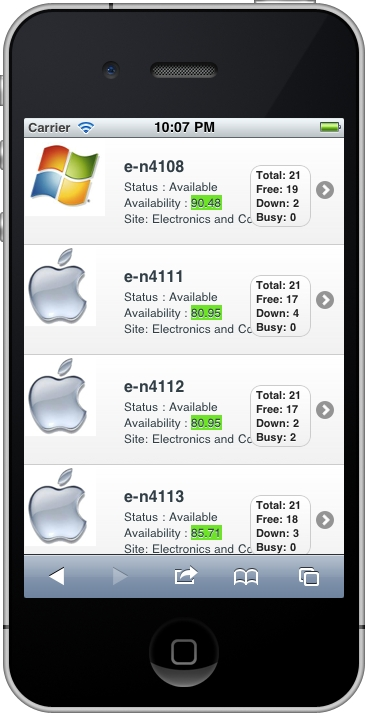
\includegraphics[scale=0.25]{phone.jpg}}
		\qquad
		\subfloat{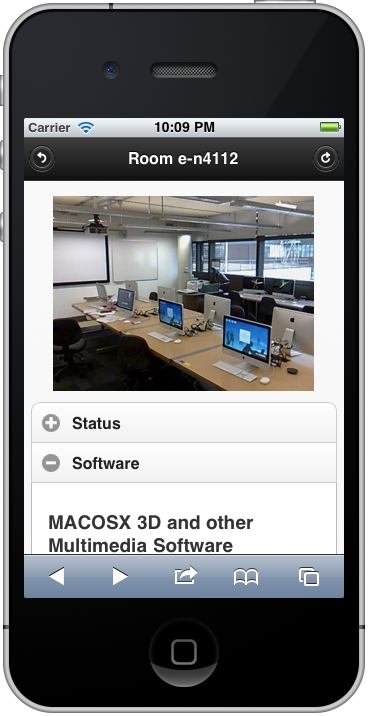
\includegraphics[scale=0.25]{phone1.jpg}}

	\end{figure}
	
\end{frame}

%%%%%%%%%%%%%%%%%%%%%%%%%%%%%%%%%

\subsection{Probl\`emes rencontr\'es}
	
\begin{frame}{Probl\`emes rencontr\'es}
	\begin{block}{Probl\`emes rencontr\'es}
		\begin{itemize}
			\item Manque de connaissances au d\'ebut
			\item Configuration SSL difficile
			\item Normalisation des informations de l'Universit\'e
			
		\end{itemize}

	\end{block}
	
\end{frame}




\chapter{Bilan}

\section{Bilan du travail r\'ealis\'e}

Ce bilan r\'esumera le travail r\'ealis\'e durant le stage.
Dans une premi\`ere partie, un r\'ecapitulatif du projet sera donn\'e, avec notamment un graphique afin de montrer les fonctionnalit\'es reprises de {\Yuukou} ainsi que les diff\'erentes fonctionnalit\'es qu'apporte {\YuukouII}.
Ensuite le calendrier des 16 semaines de stage, avec les diff\'erentes t\^aches effectu\'ees semaines apr\`es semaines.
Il sera suivi par une partie donnant ce qu'apporte le projet \`a l'Universit\'e, les avantages qu'elle peut en tirer.
Enfin une derni\`ere partie traitera des am\'eliorations qu'il est possible d'apporter au service Web afin d'accro\^itre ses performances et ses fonctionnalit\'es.

\subsection{R\'ecapitulatif du projet}

La figure~\ref{figure:yuukouEtYuukouII} permet de donner une vue d'ensemble sur les principales fonctionnalit\'es dont le projet dispose.
Les cadres pleins repr\'esentent des fonctionnalit\'es dont le principe a \'et\'e repris de {\Yuukou}, les cadres en pointill\'es, quant \`a eux, repr\'esentent les nouvelles fonctionnalit\'es qu'apporte \YuukouII.

\clearpage

\begin{figure}[!ht]
	\centering
	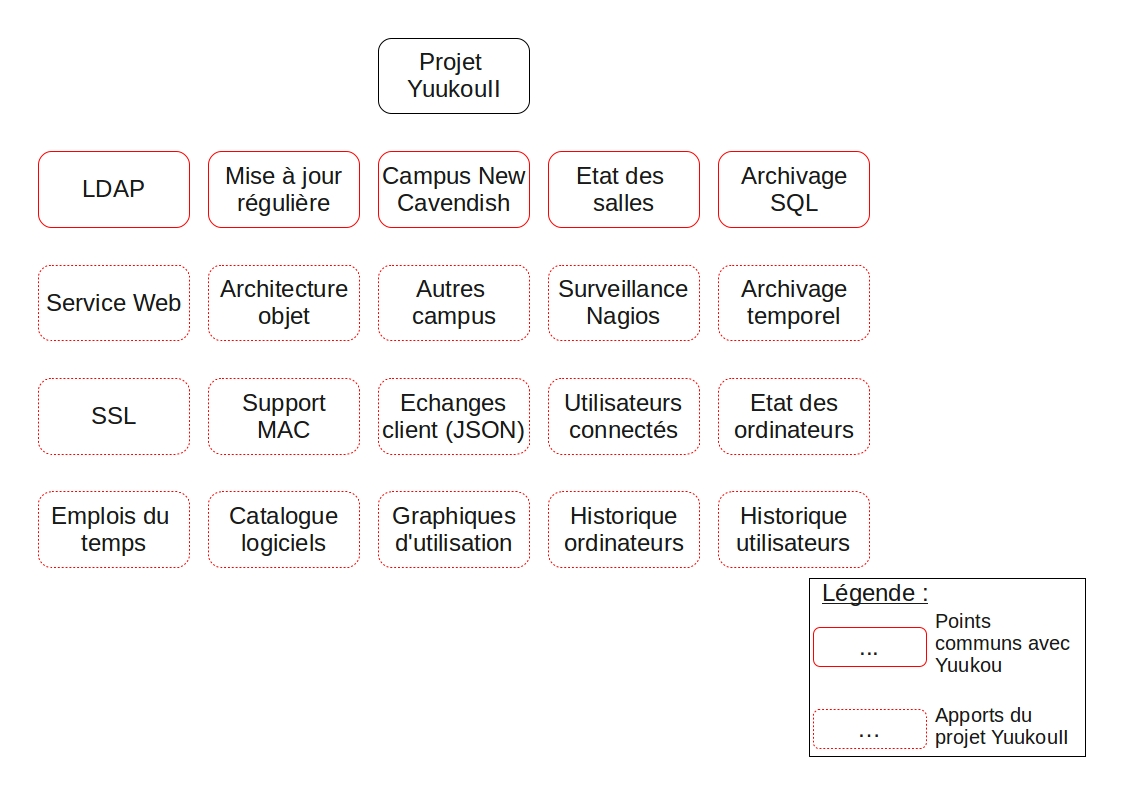
\includegraphics[scale=0.375]{yuukouEtYuukouII.jpg}
	\caption{R\'ecapitulatif des fonctionnalit\'es reprises de {\Yuukou} et les nouvelles de \YuukouII}
	\label{figure:yuukouEtYuukouII}

\end{figure}

\subsection{Calendrier du stage}

Voici le calendrier du stage d'une dur\'ee de 16 semaines commen\c{c}ant le 13 f\'evrier 2012 et terminant le 4 juin 2012.
Certains points ont demand\'e plus de travail que d'autres, comme la conception du cycle principal du service Web ou encore la mise en place du SSL qui a pos\'ee quelques difficult\'es.

\begin{description}
	\item[semaine 1] : Arriv\'ee et d\'ecouverte du projet, premier entretien avec l'\'equipe technique et leurs attentes;
	\item[semaine 2] : D\'ecouverte des services Web et choix des outils utilis\'es;
	\item[semaine 3 et 4] : Conception de la base de donn\'ees et impl\'ementation du cycle principal de l'application;
	\item[semaine 5] : Mise en place de l'emploi du temps et d\'ebut mise en place de SSL;
	\item[semaine 6] : Mise en place du syst\`eme JSON et fin de mise en place de SSL;
	\item[semaine 7 et 8] : D\'eveloppement des m\'ethodes Web;
	\item[semaine 9] : Mise en place de l'architecture finale et d\'eveloppement des m\'ethodes Web;
	\item[semaine 10] : D\'ebut de r\'edaction du rapport (pr\'esentation et sujet);
	\item[semaine 11] : D\'eveloppement des m\'ethodes Web;
	\item[semaine 12 et 13] : R\'ecup\'eration du catalogue de logiciels de M\'ediaWiki;
	\item[semaine 14] : Ajout de m\'ethodes Web et am\'elioration du syst\`eme de chargement de la base de donn\'ees;
	\item[semaine 15] : R\'edaction du rapport de stage et maintenance des fonctionnalit\'es du service Web;
	\item[semaine 16] : Fin d'\'ecriture du rapport de stage.

\end{description}

\subsection{Bilan pour l'Universit\'e}

Le service Web est fonctionnel \`a l'Universit\'e.
Il dispose d'un cycle principal permettant la r\'ecup\'eration des donn\'ees de Nagios et le stockage dans la base de donn\'ees.
De nombreuses fonctionnalit\'ees ont \'et\'e d\'evelopp\'ees pour \'etendre les possibilit\'es du service Web.
Une s\'ecurisation des communications avec la mise en place du protocole SSL.
Une gestion des emplois du temps en r\'ecup\'erant quotidiennement les diff\'erents emplois du temps des campus de l'Universit\'e.
Une gestion de la configuration logicielle des salles informatiques avec l'extraction des donn\'ees pr\'esentes sur le \textit{MediaWiki} de la \textit{School of Electronics and Computer Science}.
Une g\'en\'eration d'un graphe d'utilisation des salles informatiques dans une p\'eriode donn\'ee.

Le service Web dispose de nombreuses fonctions permettant \`a un client de r\'ecup\'erer juste les informations dont il a besoin concernant la disponibilit\'e des salles en temps r\'eel.
Mais aussi les historiques dans le temps des connexions.
Il propose aussi une gestion de cycle permettant de l'arr\^eter et de le remettre en marche.

L'utilisation de JSON permet la cr\'eation de client ind\'ependamment du langage employ\'e.
Une fois la structure du fichier retourn\'e comprise, il est facile d'extraire les donn\'ees voulues et de les afficher.

Ajout\'e \`a cela la documentation Java (\textit{javadoc}) du service Web afin que dans le futur diff\'erentes am\'eliorations, parmi celles exprim\'ees au \S~\ref{section:amelioration}, soient mises en place.

\subsection{Am\'eliorations possibles}
\label{section:amelioration}

Le projet {\YuukouII} est loin d'\^etre fini m\^eme si fonctionnel \`a l'heure actuelle.
Il reste diverses fonctionnalit\'es \`a d\'evelopper.
Une de ces fonctionnalit\'es serait de rajouter une s\'ecurit\'e lors de l'acc\`es aux m\'ethodes du service Web par le client.
En effet, il serait int\'eressant que le client s'authentifie.
De ce fait, deux r\^oles pourraient \^etre d\'efinis : administrateur et utilisateur.
Avec cette m\'ethode, un utilisateur ne pourrait jamais se servir d'une m\'ethode dite priv\'ee car actuellement, si un client d\'eveloppe son propre programme pour acc\'eder au service Web {\YuukouII}, une fois le protocole SSL en place, rien ne l'emp\^eche d'utiliser les fonctions qu'il veut.

Des am\'eliorations peuvent aussi \^etre port\'ees sur la fa\c{c}on dont RRDtool a \'et\'e mis en place.
Il ne s'agit que d'un essai pour tester les possibilit\'es, mais il serait int\'eressant de l'int\'egrer pleinement au service Web et surtout au cycle principal d'ex\'ecution.
De ce fait, les donn\'ees seraient enregistr\'ees en temps r\'eel et les requ\^etes de g\'en\'eration de graphe pourraient gagner en rapidit\'e d'ex\'ecution.
De plus, cette m\'ethode rendrait une utilisation normale de RRDtool au service Web.

La suite concernerait les attentes pour les emplois du temps et le catalogue logiciels.
En effet, la gestion des emplois du temps est susceptible d'\'evoluer vers une notation plus lisible des salles par le service responsable de la cr\'eation des emplois du temps.
Cela permettrait un suivi de toutes les salles informatiques au lieu de seulement certaines actuellement situ\'ees \`a la \textit{School of Electronics and Computer Science}.
Pour le catalogue de logiciels, le principe est un peu le m\^eme.
Ne concernant que la \textit{School of Electronics and Computer Science}, il serait int\'eressant de trouver une fa\c{c}on simple de r\'ecup\'erer les informations sur la configuration logicielle des autres salles.
Par exemple, si une partie de la base de donn\'ees permettant de construire cette configuration, en amont, pouvait \^etre disponible, l'extraction des donn\'ees s'en verrait simplifi\'ee et plus compl\`ete du fait qu'elle serait effective pour toutes les salles surveill\'ees par Nagios.

Il pourrait aussi \^etre impl\'ement\'e une s\'erie de petites fonctions permettant d'effectuer des modifications d'informations, quand le service Web est en maintenance, sur les diff\'erentes tables.
Par exemple l'ajout d'une salle avec l'aide d'une interface Web.

Nagios surveille actuellement les salles informatiques de l'Universit\'e, cependant, il est possible de lui faire surveiller les imprimantes et d'ajouter les services adapt\'es comme la gestion du niveau d'encre et du papier.
Un \'etudiant recherchant une imprimante de libre obtiendrait les salles correspondantes.
Avec cela, il serait possible d'avoir un statut complet d'une salle informatique.

Il serait aussi int\'eressant d'ajouter des fonctions au service Web pour retourner les informations sur la surveillance des salles sous forme d'un flux RSS$^*$ pouvant \^etre exploit\'e de fa\c{c}on diff\'erente par un client.


\section{Bilan personnel}

D'un point de vue humain, ce stage m'a beaucoup apport\'e, sp\'ecialement au niveau de la langue.
Je me suis rendu compte combien il est difficile au d\'ebut de communiquer convenablement avec quelqu'un.
Le m\^eme cycle se r\'ep\`ete : on essaye de traduire ce que l'on entend, ensuite on r\'efl\'echi \`a la r\'eponse en fran\c{c}ais, on la traduit rapidement et on la dit plus ou moins bien.
C'est compliqu\'e de se d\'efaire de ce cycle mais apr\`es quelques mois, j'ai pu ressentir beaucoup plus de facilit\'e \`a communiquer avec les membres du CPC.

De plus, je suis vraiment content d'avoir pu effectuer mon stage dans une ville si cosmopolite que Londres.
J'ai pu y d\'ecouvrir une vie un peu diff\'erente de celle que je connaissais.
Durant les quatre mois, j'ai r\'esid\'e dans une r\'esidence \'etudiante o\`u j'ai partag\'e une chambre avec un croate, de ce fait, je n'avais pas d'autre choix que de parler anglais avec lui.
C'\'etait d'autant plus le cas que la majorit\'e des r\'esidents n'\'etaient pas anglais, mais venaient d'un peu partout dans le monde.
Chose qui, je pense, m'a beaucoup fait progresser notamment dans le parl\'e, tout en gardant quand m\^eme un fort accent fran\c{c}ais.

Concernant le cadre du stage, j'ai beaucoup appr\'eci\'e la prise en charge de M. DELAITRE qui s'est beaucoup impliqu\'e dans ce projet, tant dans la partie service Web que dans la partie affichage.
J'ai r\'eellement aim\'e la libert\'e d'action qu'il m'a laiss\'e dans le projet tout en fixant les objectifs qu'il voulait voir accompli.

La collaboration avec les diff\'erents acteurs du projet d'affichage s'est tr\`es bien pass\'ee, notamment avec M. Yacine MAGHEZZI comme nous \'etions dans le m\^eme bureau.
Nous avons d\^u beaucoup discuter l'un avec l'autre concernant le retour d'informations du service Web.
Mon objectif \'etait vraiment de faciliter un maximum le travail des autres d\'eveloppeurs pour qu'ils puissent se concentrer essentiellement sur la partie affichage.

D'un point de vue p\'edagogique, ce stage fut vraiment tr\`es riches en nouvelles connaissances.
J'ai pu y d\'ecouvrir les services Web que je ne connaissais pas auparavant ainsi que des outils qui m'\'etaient totalement inconnus comme NetBeans et GlassFish.
J'avoue avoir des appr\'ehensions quand on me parle de technologies du Web mais le projet que m'a confi\'e M. Thierry DELAITRE m'a vraiment passionn\'e du d\'ebut \`a la fin du stage.
J'ai pu r\'eutiliser beaucoup de mes acquis avec le d\'eveloppement Java, les interactions avec les bases de donn\'ees ou encore la manipulation de fichiers XML.



\clearpage


\chapter{Conclusion}

Ce stage de deuxi\`eme ann\'ee de Master informatique est une chance de se projeter dans le contexte d'un travail r\'eel en entreprise en travaillant avec des technologies du march\'e.
La libert\'e dont j'ai b\'en\'efici\'e durant toute la dur\'ee du stage m'a permis de d\'ecouvrir de nouvelles technologies et le concept des services Web notamment.
J'ai pu remettre en question certains de mes choix et exercer un avis critique sur mon travail pour au final fournir un service Web fonctionnel.
Celui-ci comprend un cycle principal permettant la r\'ecup\'eration d'informations issues de Nagios pour les stocker dans une base de donn\'ees, ainsi que de multiples fonctions permettant \`a un client d'extraire une partie des donn\'ees qui peuvent lui \^etre utiles afin de pouvoir v\'erifier la disponibilit\'e des salles informatiques dans l'Universit\'e de Westminster.

Ce travail a \'et\'e aussi une chance de travailler en \'equipe avec diff\'erentes personnes.
La communication fut tr\`es importante tout au long du d\'eveloppement afin de pouvoir se mettre d'accord et arriver \`a un r\'esultat tant pour la partie service Web que pour la partie affichage.
Au final, l'application cliente est capable d'afficher toutes les informations concernant la disponibilit\'e des salles en prenant en compte l'emploi du temps.
Elle fournit aussi aux membres des \'equipes techniques des informations suppl\'ementaires comme des graphiques ou des r\'esum\'es sur la situation globale des salles informatiques de l'Universit\'e.

Le stage fut aussi une bonne opportunit\'e d'am\'eliorer mon anglais.
\'Etant dans un environnement en grande partie anglophone, ma compr\'ehension et ma pratique de la langue n'en ont \'et\'e que meilleures.
Ce fut aussi la premi\`ere fois que je venais dans cette ville, j'ai donc pu la d\'ecouvrir ainsi que les diff\'erents modes de vie qui la composent.

Je suis au final tr\`es satisfait de ce stage qui m'a apport\'e beaucoup de connaissances ainsi qu'une meilleure pratique de l'anglais.
L'application est disponible actuellement pour les membres de l'Universit\'e.
Il reste encore beaucoup de travail dessus et les possibilit\'es pouvant l'enrichir sont tr\`es nombreuses.

\clearpage


\end{document}
